\section{Real-World Deployment of DSpark}   
\label{sec:real_world_deployment}  

While \autoref{sec:experiments} establishes the algorithmic gains of DSpark on offline benchmarks, deploying it alongside large-scale models like DeepSeek-V4~\citep{deepseekai2026deepseekv4highlyefficientmilliontoken} introduces additional system-level challenges across both training and inference. In this section, we present the end-to-end production pipeline of DSpark. We detail our scalable training mechanisms, the system-level optimizations necessary to deploy the hardware-aware prefix scheduler~(\autoref{sec:scheduler}), and the framework's end-to-end performance under live user traffic.

\subsection{Scalable and Flexible Training}   
\label{sec:prod_training}  
  
The DSpark draft models are co-deployed with the preview versions of DeepSeek-V4-Flash and DeepSeek-V4-Pro~\citep{deepseekai2026deepseekv4highlyefficientmilliontoken}. The parallel backbone comprises three MoE layers~\citep{dai2024deepseekmoe} with mHC~\citep{xie2025mhc} and a sliding window attention of 128. We configure the maximum block size to $\gamma=5$ and utilize the Markov head for sequential modeling. 
Furthermore, the confidence head is trained end-to-end alongside the draft model and subsequently calibrated via STS to provide reliable scheduling signals.
  
Training the draft model requires the target model's output distributions for supervision. Evaluating both models over the full document context incurs substantial memory footprints and inter-worker communication overhead. To address these bottlenecks, we implement two system-level optimizations within our internal training framework~(HAI-LLM)\footnote{\url{https://www.high-flyer.cn/en/blog/hai-llm/}}:

\begin{itemize}[leftmargin=*,itemsep=4pt,topsep=4pt]   
    \item \textbf{Hidden state communication.} Transferring the target model's full-vocabulary logits ($V \approx 10^5$) across parallel workers creates a significant bandwidth bottleneck. Instead, we temporarily cache the target model's forward-pass activations and communicate only the hidden states immediately preceding the language modeling (LM) head. The LM head projection is then executed locally on the draft model's workers only for the sampled target positions. This reduces the per-token communication complexity to $O(d)$, where $d$ is the hidden dimension.
      
    \item \textbf{Anchor-bounded sequence packing.} To decouple the draft model's computational cost from the target model's context length, we sample a fixed number of draft anchors from the training sequence and pack these isolated prediction blocks into dense training batches. We manage this packing via token-level attention indices rather than standard 2D masks. This maintains exact causal masking across multiple independent sequences and anchors, avoiding the computational and memory overhead associated with standard padding.  
\end{itemize}


\subsection{Hardware-Aware Prefix Scheduler in Practice}
\label{sec:scheduler_in_practice}

In \autoref{sec:scheduler}, \autoref{alg:prefix-scheduler} provides a theoretically sound and lossless scheduling mechanism. However, directly deploying this algorithm into a production environment exposes two fundamental conflicts with real-world infrastructure. 
First, the algorithm assumes a smooth, unimodal capacity curve, whereas the true hardware capacity $\text{SPS}(B)$ is inherently discrete, exhibiting a jagged, step-wise degradation~\citep{Yan2020DemystifyingTC}. 
Second, the algorithm requires scheduling of dynamic draft tokens per step, which clashes with continuous CUDA graph replay~\citep{fireworks2023cudagraphs} and Zero-Overhead Scheduling (ZOS)~\citep{zhu2025nanoflowoptimallargelanguage,zheng2024sglangefficientexecutionstructured}. 

To navigate the trade-offs among system compatibility, throughput, and algorithmic correctness, we adapt the scheduler to operate asynchronously. Because ZOS requires the batch size for the next step to be known before the current step completes, synchronous scheduling would inevitably stall the GPU pipeline. Instead, we approximate the upcoming verification capacity using the confidence head outputs from two steps prior. Mechanically, the candidate tokens in the current step are still strictly sorted by their actual, up-to-date cumulative confidence scores; the historical prediction from two steps prior is used solely to determine the dynamic truncation length (i.e., the batch capacity limit $K$). This effectively casts the admission process as a dynamic top-$K$ selection. While approximating the capacity $K$ introduces a slight temporal offset, the selection mechanism is fundamentally rank-preserving: the most confident draft tokens are always prioritized for verification. This adaptation fully hides scheduling latency and ensures seamless ZOS integration.

Building on this asynchronous pipeline, we resolve the hardware utilization bottleneck. To prevent the scheduler from being trapped in local minima by jagged $\text{SPS}$ cliffs, we remove the early-stopping \texttt{break}, enabling an unconstrained global search. Ordinarily, this retrospective search would leak future token information and violate the lossless guarantee~(\autoref{app:counterexample}). However, our ZOS-driven adaptation naturally prevents this. Because the unconstrained search evaluates only historical predictions from two steps prior, the admission decision is isolated from the realization of the current token $x_{r,k}$. The truncation length inherently depends only on information available from two steps prior. Thus, asynchronous design forms a causal barrier, maximizing physical throughput across hardware cliffs while preserving the exact target distribution.

\subsection{High-Throughput and Low-Latency Inference} 
\label{sec:prod_systems}

During decoding, production serving systems must simultaneously optimize two competing objectives: per-request latency and aggregate throughput~\citep{kwon2023efficient,zhong2024distserve,zhao2025insights}. The former governs the quality of service for individual users---a factor increasingly critical in agent-based workloads~\citep{tiwari2026cachewise}---while the latter determines the total number of concurrently served users. Because speculative decoding inevitably incurs wasted verification compute, it inherently navigates this trade-off, trading extra system compute for faster per-request generation. 

In our deployment setting, however, the number of requests processed per step is frequently constrained by resource limits (e.g., fixed KV-cache capacity per request) and the pool of available user traffic (e.g., RL long-tail loads). Consequently, the effective batch size persistently remains well below the GPU's compute-saturating threshold. 
Under this regime, the traditional trade-off simplifies: given a fixed concurrency limit, maximizing per-GPU total token throughput and maximizing the generation speed per user~(\textit{tok/s/user}) become highly correlated objectives rather than competing ones.

To achieve this maximum throughput, the asynchronous scheduler (\autoref{sec:scheduler_in_practice}) actively routes idle compute toward the most promising draft tokens. However, executing this dynamic routing introduces a severe challenge at the physical execution layer: the inference framework must efficiently support variable-length queries within a single batch. Standard decode kernels are heavily optimized for fixed query lengths; naively processing variable-length verified prefixes leads to severe GPU under-utilization due to padding and uneven workload distribution. We resolve this by decoupling physical execution from logical sequence tracking. In our compute kernels, all tokens across different requests are flattened and processed identically as independent elements. The complex intra-sequence dependencies are then strictly conveyed via a marker tensor integrated into our sparse attention implementation. Specifically on the DeepSeek-V4 architecture, only the index-attention and compress kernels require modification to support this variable-length routing, allowing the dynamic scheduler to operate seamlessly without introducing low-level execution overhead.

\subsection{Performance under Live User Traffic}
\label{sec:prod_evaluation}

\begin{figure}[thbp!] 
\centering
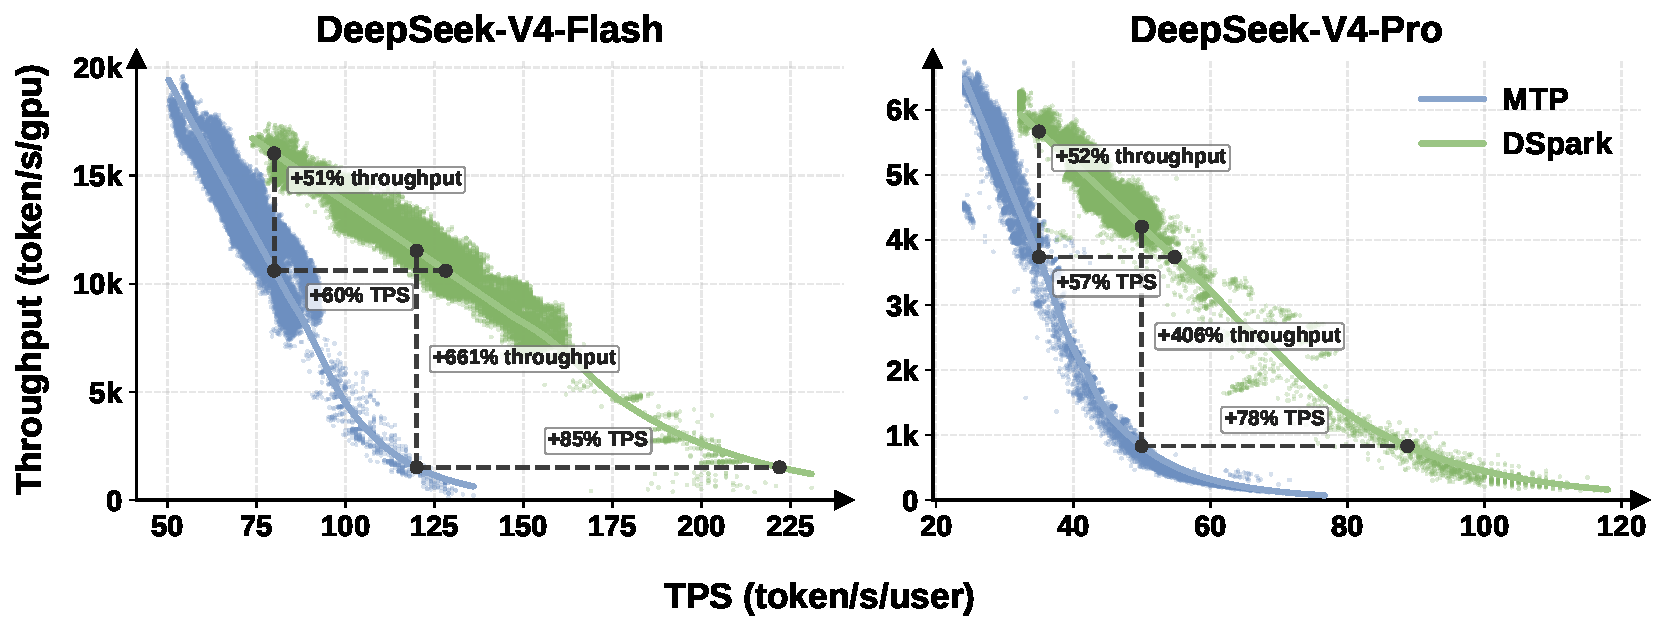
\includegraphics[width=\linewidth]{figs/online_service.pdf} 
\caption{
\textbf{Throughput vs.\ TPS.} 
Aggregate output token throughput against per-request generation speed (tok/s/user) under live traffic. 
In our production deployment, DSpark improves the observed throughput–interactivity frontier relative to the MTP-1 baseline under the measured traffic and engine configurations.
} 
\label{fig:prod-interactivity} 
\end{figure} 

We evaluate DSpark-5 (configured with a maximum draft length of $\gamma=5$) against the MTP-1~\citep{liu2024deepseek} baseline within the production serving engines of DeepSeek-V4-Flash~(preview) and DeepSeek-V4-Pro~(preview).
MTP-1 represents the former production setup, having been superseded by DSpark two weeks following the DeepSeek-V4-preview release.
This single-token setup was historically maintained in production because deploying a static multi-token drafter (e.g., MTP-3/5) strictly degrades aggregate throughput under high concurrency due to excessive verification overhead. 
Therefore, comparing DSpark against this established baseline directly demonstrates its ability to safely unlock the performance potential of larger draft blocks in dynamic serving environments. 
In all figures, the scatter points represent raw telemetry data sampled directly from live user traffic, capturing complex, real-world request distributions, while the solid lines represent the fitted performance frontiers.

\paragraph{The Serving Pareto Frontier.}
\autoref{fig:prod-interactivity} illustrates the trade-off between aggregate system throughput and per-user generation speed (interactivity).
To quantify DSpark's behavior under practical deployment constraints, we evaluate the system at several interactivity SLA anchors. Here, an SLA (Service Level Agreement) specifies the minimum per-user generation speed (in tokens per second) that the system must guarantee.

For the V4-Flash engine, we evaluate the system at SLA anchors of 80 and 120 tok/s/user. 
At the moderate 80 tok/s/user SLA, DSpark improves aggregate throughput by 51\% over the MTP-1 baseline.
The stricter 120 tok/s/user SLA represents a qualitatively different regime: under this constraint, the single-token MTP-1 baseline approaches its operational boundary and can sustain only a very small concurrent batch.
Consequently, the relative throughput ratio at this point is numerically large, with DSpark achieving a nominal 661\% higher aggregate throughput.
We therefore interpret this high-SLA point primarily as evidence that DSpark extends the feasible interactivity frontier, rather than as a representative multiplicative speedup over a well-utilized baseline.
At matched practical throughput levels, which provide a more stable comparison, DSpark accelerates per-user generation speeds by 60\% to 85\%.

The V4-Pro deployment shows the same pattern.
At the moderate 35 tok/s/user SLA, DSpark improves aggregate throughput by 52\%.
At the stricter 50 tok/s/user SLA, MTP-1 again enters a low-concurrency regime, yielding a nominal 406\% relative throughput advantage for DSpark.
As with V4-Flash, we treat this point as an indication that DSpark sustains useful throughput under an interactivity target that the baseline cannot efficiently support.
At matched system capacities, DSpark delivers 57\% to 78\% faster per-user generation.
Overall, these results show that DSpark shifts the observed throughput--interactivity frontier outward: it improves throughput in moderate-SLA regimes and, more importantly, preserves non-degenerate serving capacity under strict interactivity constraints.

\paragraph{Throughput Dynamics under Load.}

\begin{figure}[thbp!]   
\centering  
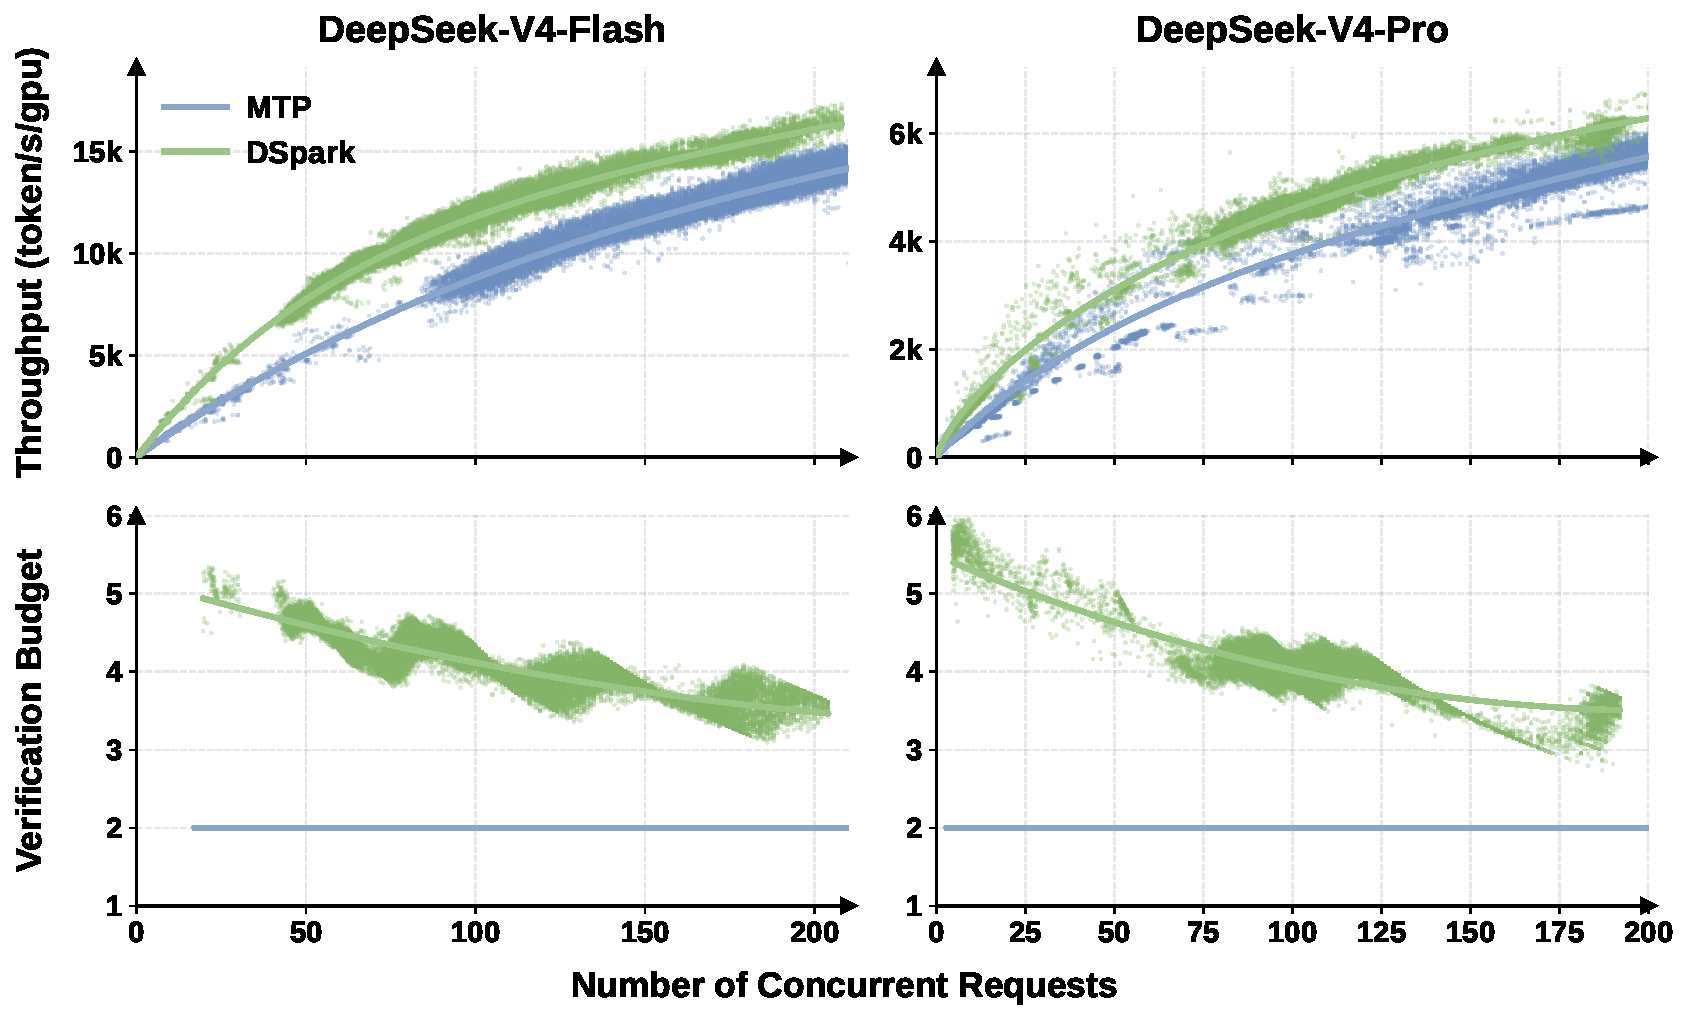
\includegraphics[width=0.9\linewidth]{figs/online_service_tradeoff.pdf}   
\caption{\textbf{Load-adaptive throughput and verification budgets.} Top row (a, b): Aggregate output throughput across varying levels of system concurrency. Bottom row (c, d): The average target verification budget allocated per request. As concurrent load increases, the dynamic scheduler automatically restricts the per-request verification length to prevent resource contention.}   
\label{fig:prod-scalability}   
\end{figure}

\autoref{fig:prod-scalability} analyzes the underlying mechanism driving these gains by plotting aggregate throughput (top row) and the dynamic verification budget (bottom row) against system concurrency.
\begin{itemize}
    \item Under the moderate concurrency regimes typical of our production deployment (fewer than 200 concurrent requests for V4-Flash and 150 for V4-Pro), the hardware-aware scheduler leverages available target compute capacity by allocating longer verification budgets, expanding from MTP-1's static 2 tokens to roughly 4--6 tokens per request. This extended verification yields more accepted tokens per forward pass, directly contributing to the throughput gains observed on the Pareto frontier.
    \item As system concurrency scales and target capacity saturates, the scheduler dynamically restricts this budget. The average verification length decreases smoothly with load, ensuring that low-confidence draft tokens are pruned before they consume critical batch capacity. This load-aware behavior stabilizes production deployment: DSpark maximizes the utility of idle compute under light traffic, while effectively preserving critical batch capacity under heavy traffic.
\end{itemize}

\paragraph{Limitations.}Although the prefix scheduler minimizes wasted target-model verification, DSpark still incurs a fixed draft-side cost to generate the initial $\gamma$-token block via the parallel backbone. For complex queries with inherently low acceptance rates, this upfront drafting compute is unrecoverable. Future optimizations could introduce difficulty-aware early exiting within the draft model, enabling such requests to bypass full-block generation.